\usetikzlibrary{arrows.meta}
\begin{frame}{SOCKS (RFC 1928)}
    \begin{itemize}
    \item SOCKS motivation in RFC: firewall traversal
    \item supports both TCP and UDP
    \end{itemize}
\end{frame}

\begin{frame}{SOCKS TCP operation (client)}
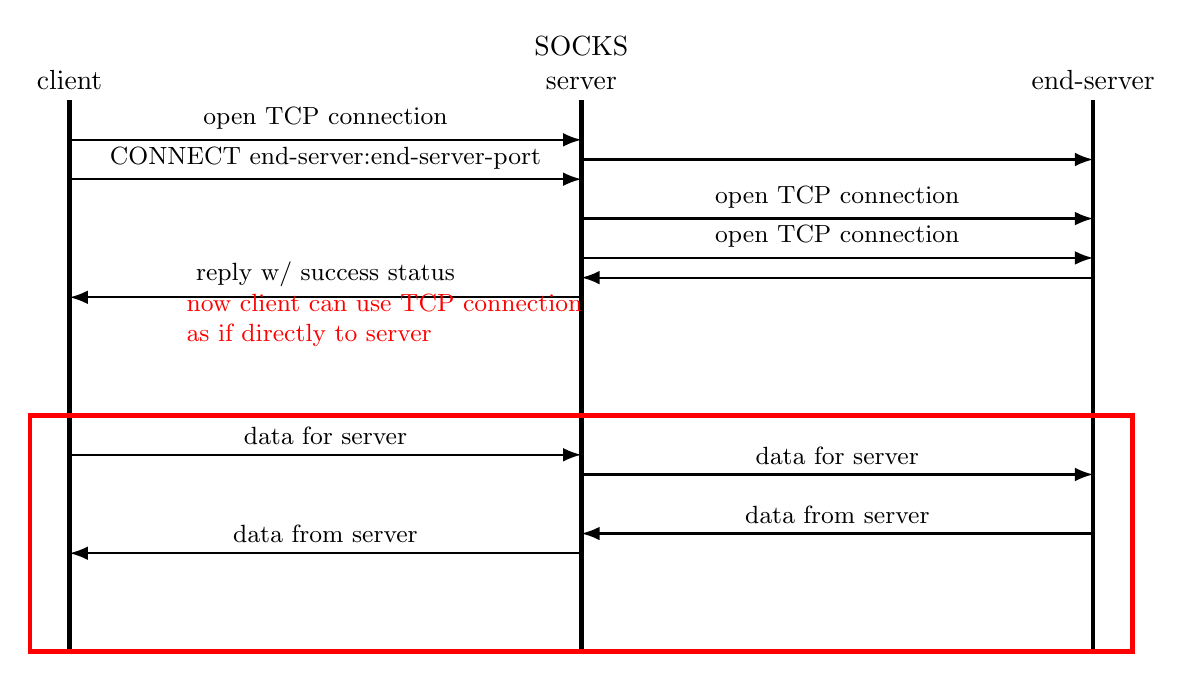
\begin{tikzpicture}
\begin{scope}[ultra thick]
    \draw (0, 0) node[above] {client} -- ++(0, -7);
    \draw (6.5, 0) node[above,align=center] {SOCKS\\server} -- ++(0, -7);
    \draw (13, 0) node[above] {end-server} -- ++(0, -7);
\end{scope}
\tikzset{
    msg/.style={font=\small},
    send/.style={thick,-Latex},
}
\draw[send] (0, -.5) -- ++(6.5, 0) node[midway,above,msg] {open TCP connection};
\draw[send] (6.5, -.75) -- ++(6.5, 0);
\draw[send] (0, -1) -- ++(6.5, 0) node[midway,above,msg] {CONNECT end-server:end-server-port};
\draw[send] (6.5, -1.5) -- ++(6.5, 0) node[midway,above,msg] {open TCP connection};
\draw[send] (6.5, -2) -- ++(6.5, 0) node[midway,above,msg] {open TCP connection};
\draw[send] (13, -2.25) -- ++(-6.5, 0);
\draw[send] (6.5, -2.5) -- ++(-6.5, 0) node[midway,above,msg] {reply w/ success status};
%
\draw[ultra thick,red] (-.5, -4) rectangle (13.5, -7);
\node[align=left,anchor=south,font=\small,red] at (4, -3.25) {
    now client can use TCP connection \\ as if directly to server
};
\draw[send] (0, -4.5) -- ++(6.5, 0) node[midway,above,msg] {data for server};
\draw[send] (6.5, -4.75) -- ++(6.5, 0) node[midway,above,msg] {data for server};
\draw[send] (13, -5.5) -- ++(-6.5, 0) node[midway,above,msg] {data from server};
\draw[send] (6.5, -5.75) -- ++(-6.5, 0) node[midway,above,msg] {data from server};
\end{tikzpicture}
\end{frame}

\begin{frame}{SOCKS TCP operation (server)}
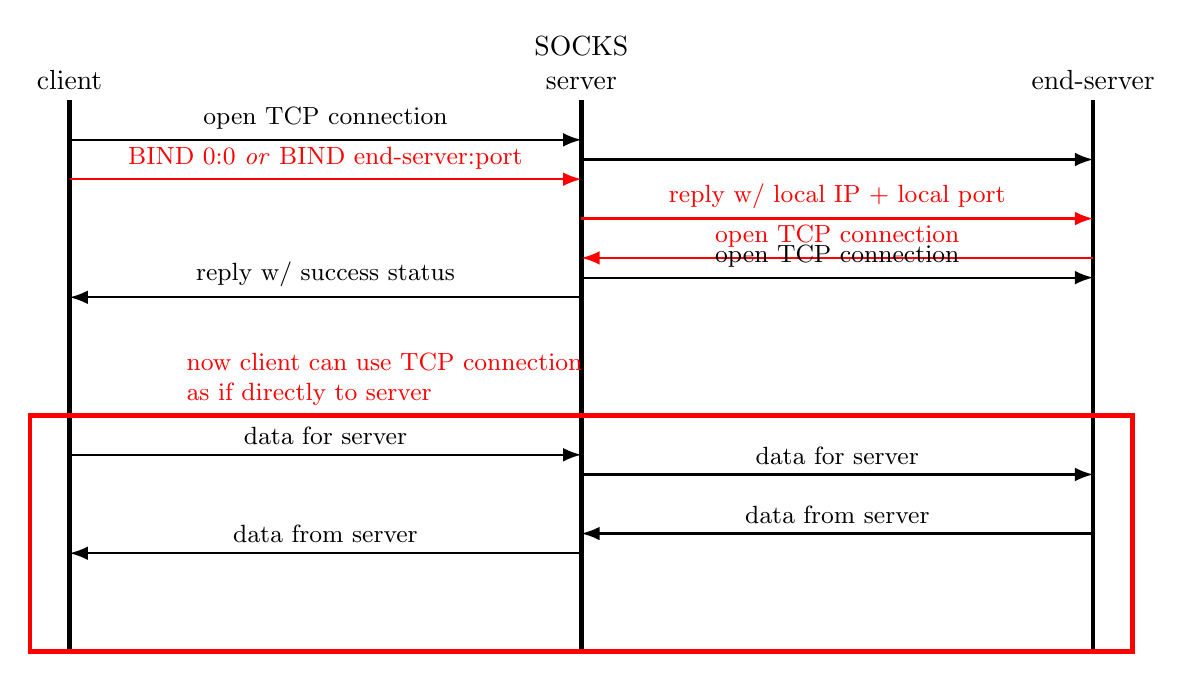
\begin{tikzpicture}
\begin{scope}[ultra thick]
    \draw (0, 0) node[above] {client} -- ++(0, -7);
    \draw (6.5, 0) node[above,align=center] {SOCKS\\server} -- ++(0, -7);
    \draw (13, 0) node[above] {end-server} -- ++(0, -7);
\end{scope}
\tikzset{
    msg/.style={font=\small},
    send/.style={thick,-Latex},
    send misc/.style={thick,dotted,-Latex},
}
\draw[send] (0, -.5) -- ++(6.5, 0) node[midway,above,msg] {open TCP connection};
\draw[send] (6.5, -.75) -- ++(6.5, 0);
\draw[red,send] (0, -1) -- ++(6.5, 0) node[midway,above,msg] {BIND 0:0 \textit{or} BIND end-server:port};
\draw[red,send] (6.5, -1.5) -- ++(6.5, 0) node[midway,above,msg] {reply w/ local IP + local port};
\draw[red,send] (13, -2) -- ++(-6.5, 0) node[midway,above,msg] {open TCP connection};
\draw[send] (6.5, -2.25) -- ++(6.5, 0) node[midway,above,msg] {open TCP connection};
\draw[send] (6.5, -2.5) -- ++(-6.5, 0) node[midway,above,msg] {reply w/ success status};
%
\draw[ultra thick,red] (-.5, -4) rectangle (13.5, -7);
    \node[align=left,anchor=south,font=\small,red] at (4, -4) { now client can use TCP connection \\ as if directly to server };
\draw[send] (0, -4.5) -- ++(6.5, 0) node[midway,above,msg] {data for server};
\draw[send] (6.5, -4.75) -- ++(6.5, 0) node[midway,above,msg] {data for server};
\draw[send] (13, -5.5) -- ++(-6.5, 0) node[midway,above,msg] {data from server};
\draw[send] (6.5, -5.75) -- ++(-6.5, 0) node[midway,above,msg] {data from server};
\end{tikzpicture}
\end{frame}

\begin{frame}[fragile,label=udpSocks]{SOCKS UDP operation}
    \begin{itemize}
    \item use TCP to get UDP port for proxy to use
    \item send/receives UDP packets with ``request header'':
    \end{itemize}
\begin{Verbatim}
      +----+------+------+----------+----------+----------+
      |RSV | FRAG | ATYP | DST.ADDR | DST.PORT |   DATA   |
      +----+------+------+----------+----------+----------+
      | 2  |  1   |  1   | Variable |    2     | Variable |
      +----+------+------+----------+----------+----------+
\end{Verbatim}
    \begin{itemize}
    \item FRAG = which fragment number
        \begin{itemize}
        \item added header means we might need to split UDP packets up
        \item 0 = not fragmented, most sig bit = last fragment
        \end{itemize}
    \item ATYP = address type (IPv4/IPv6/DNS name)
    \end{itemize}
\end{frame}
